\section{On-path serialization}

In this section, we show an on-path serializer can address both the
the performance bottlenecks associated with RDMA hardware and the
overhead of remote conflict resolution.  First, we describe how to
accelerate locking as used in Sherman by leveraging the ability to
rewrite RDMA requests after their ordering is determined to replace
expensive CAS requests with simple write verbs and rely upon the
semantics of RDMA RC queue pairs to provide serializability.
%Additionally, we can leverage
%this same functionality to multiplex independent operations across multiple QP
%to improve scalability.
Second we show how even imperfect knowledge of the instruction ordering
can be used to avoid most---but not necessarily all---conflicts by
modifying operations in flight, thereby avoiding Clover's expensive
conflict resolution machinery in many cases.

%describe how to effectively do away with the
%need for most retries by ``fixing'' operations issued with stale hints in
%flight.  

%% \subsection{System overview}

%% \todo{total rewrite}
%% Any asynchronous data structure which allows for lock-less reads and
%% writes must have a mechanism in place to resolve conflicts. When
%% memory is close, conflict resolution strategies can make many reads
%% and writes quickly; in the uncommon case of a conflict, the cost of
%% resolution is typically amortized by the unlikelihood of the conflict
%% itself. In the case of far memory the cost of a conflict is severe. In
%% contrast to opportunistic algorithms in a shared-cache architecture,
%% in a rack-scale disaggregated system conflicts can be detected at the
%% top-of-rack switch and resolved in the data path. Our solution,
%% \sword, leverages programmable ToR switches to allow developers with
%% knowledge of the disaggregated memory protocol to resolve conflicts
%% transparently in flight as the operations flow traverse the ToR.

\subsection{Enforcing ordering}
\label{ea}

If {\sword} is able to ensure that requests will not be reordered between when
it operates on them and their arrival at a memory server---because, for example,
it is directly connected over a single link---we can leverage the ordering
semantics provided by RDMA queue pairs to completely eliminate data races.
%%
In that case, there is no need to incur the expense of RDMA atomic
requests; {\sword} can simply replace them with lightweight verbs to
dramatically increase the scalability of a given memory server.
Importantly, this optimization can be applied selectively to only the
set of servers (or memory ranges, i.e., locks) for which {\sword} is
suitably located and sufficiently provisioned to manage; atomic
operations destined for other servers and/or memory addresses can be
left unmodified.

\subsubsection{Shared locks}
\label{sec:locking-algorithm}

One common way to limit the impact of expensive RDMA atomics is to use
them to guard only a subset of the remote data.  For example, Sherman
uses CAS operations to implement its node locks.
%Sherman and future far memory systems like Sherman which use lock based
%approaches to guard remote data will incur the cost of using RDMA atomics. 
%
%Implementing locks with CAS is straightforward, the following algorithm is
%common and is used to implement locks for nodes in Sherman. The
%CAS operations are of the form \texttt{CAS(old\_value,new\_value)}.
Sherman's locks are simply specific (NIC-hosted) memory locations
that store either a one (locked) or zero (free).  Hence, lock requests
are expressed as \texttt{CAS(0,1)}, which fail if the lock is
unavailable (i.e., the stored value is currently not 0) or atomically
set the value to 1---acquiring the lock---if successful. Unlock
operations are the inverse.

Presuming communication between the ToR and the memory server is
reliable and in-order (as provided by an RDMA QP), it is conceptually
straightforward for \sword\ to cache the current value of the lock at
the ToR.  Indeed, one could implement the lock server at the ToR
itself~\cite{netlock}, but that would require a redesign of the
underlying system; our goal is to support selective deployment where
\sword\ may not be on-path for all servers, dictating that we do not
make any changes to the existing system.  Moreover, our approach does
not require terminating RDMA connections at the switch, which would
require extensive buffering.
%to support go-back-$n$ retransmissions.

%
%This technique does not reduce contention on the lock, but simply removes the
%CAS hardware bottleneck. An alternative approach to this locking scheme would b%e
%% to use the switch as a lock server similar to
%% Netlock~\cite{netlock}.~\todo{help!}Our goals are orthogonal to
%% Netlock as we want to accelerate existing protocols, not require any
%% end host code modifications, keep switch logic to a minimum, and
%% maintain only soft state on the switch. By propagating requests to
%% end hosts we ensure that no state is lost on switch failure. And
%% that any async read operations can be issued to remote memory
%% directly without needed to be interpreted by the switch.  By
%% Forwarding all requests we remove the need for the switch to
%% implement go-back-n retransmissions. The switch is only required to
%% store the current state of the lock, and track outstanding requests
%% to modify their return values. In the following section we will see
%% that tracking outstanding requests is required when swapping CAS to
%% write across multiple connections.



In our design, \sword\ uses its local cache to determine whether an
arriving CAS operation will succeed or fail.  (If it does not have the
current value at the target address cached, it allows the atomic to
pass through unmodified and populates its cache with the response.)
Moreover, \sword\ forwards all operations for a given address over the
same QP to maintain ordering between the ToR and destination server,
allowing it to replace the CAS operation with a lightweight write in
flight.  When a lock (CAS) operation arrives, the switch checks its
cache for the state of the lock. If it is unlocked, the CAS operation
is replaced with a write and forwarded over a specific QP to the
remote server. When the (successful) response comes back,
\sword\ updates its cache and converts the write response to a CAS
success response before forwarding it back over the original QP to the
client. In the case when the lock is already held, the switch still
forwards a write request to the memory server---to ensure the client
and server agree regarding the total number of RDMA verbs communicated
between them---but the response will be replaced with a CAS failure so
that the sender knows the lock acquisition failed.
%Again, unlock is similar.


% One might ask why not host all locks on the switch thereby
% reducing bandwidth to end hosts and saving latency? By forwarding all traffic to
% the memory servers, memory can still act as ground truth for the state of shared
% data. If a switch were to be reset, no lock state is lost. Further it allows for
% optimizations, clients can read shared structures and determine what data is
% locked by inspecting memory with reads directly. This saves implementing
% potentially complex read and write logic for all data structure access on the
% switch, and prevents it from becoming a single point of failure.


% The combination of read and write steering dramatically improves the
% performance of Clover (as shown in Section~\ref{s:results}), but only
% scratches the surface of the potential improvements for far memory
% systems.  


\subsubsection{Connection remapping}

Atomic replacement only works when all operations---across all client
connections---that share server state are vectored to the same queue pair.  In
general, the determination of which operations share state is application
specific and requires inspecting each packet to extract the relevant pieces
of metadata. In the case of Sherman, lock locations can be identified by
inspecting CAS requests. Each CAS virtual address corresponds to a node lock in
the Sherman B+Tree.
%%While removing locking operations is a general principle here we consider a
%%solution for RDMA.  %Different transports with different ordering guarantees
%%would require bespoke solutions.  
The challenge, of course, is that the RDMA specification stipulates that each
client establish its own queue pair with a given server, so operations for a
given lock from different clients will arrive at the ToR on distinct queue
pairs.  \sword, then, must interpose on the full set of queue pairs terminated
by a given (set of) server(s) and vector operations to queue pairs accordingly.
This seems reasonable, as the ToR is usually on-path for all servers in a rack
in traditional topologies.

\paragraph{Sequence-space stitching.}

Multiplexing and demultiplexing RDMA requests across established connections
requires significant care. Requests on a single connection must have monotonic
sequence numbers from both the sender's and receiver's perspectives. If
monotonicity is broken, the server NIC will trigger retransmission or issue
explicit congestion notifications. To ensure monotonic sequence numbers on
shared connections {\sword} tracks the outstanding sequence number per QP and
injects the appropriate sequence number into the packet after the mapping
decision has been made.  (Ironically, there is no need to ensure any particular
ordering among requests from separate clients, so any total ordering suffices.)
%% This monotonic sequence number increment and QP mapping is the %
%serialization point which replaces the use of the RDMA CAS % request. As long
%as a packet is given an atomically incremental % sequence number from our
%middle box and placed on a stateful % partitioned connection, it will execute
%in the same serialized % order as if it were protected by a CAS. We are
%guaranteed this due % to the ordering requirements of RDMA reliable
%connections.

When an RDMA request arrives at {\sword} from a client, it is
mapped to the appropriate queue pair for the relevant lock and a
\emph{stub} is stored to aid in mapping the request back, much like a
network address translator (NAT). The stub keeps track of the original
request's sequence number, IP address, MAC address, and queue
pair. Stubs are stored in an array of size $n$ indexed by their
sequence number $\pmod n$ to ensure $O(1)$ lookup when demultiplexing
the response.
%%
In addition to sequence numbers, a \emph{message} sequence number
is used as an RDMA optimization by the memory server NIC. This value
is transmitted as part of the RoCE BTH+ header in the response packet
and corresponds to the highest request number the server has
processed. If this value is wrong in the response packet from the
perspective of the sender (i.e., is less than another message sequence
number previously received by that client), the entire request is
retransmitted.  {\sword} maintains the message sequence number each client
expects to see by keeping track of the number of requests a client has
issued and adding it to the value of the original message sequence
number for that connection.

\paragraph{Request coalescing.}

As an additional complication, {\sword} must deal with the fact
that RoCE coalesces some ACKs as an optimization.  In particular
multiple RDMA requests can be acknowledged by a single
acknowledgment, in the form of either an ACK, ATOMIC ACK, or Read
Response. This occurs when multiple RDMA requests are processed
concurrently.  Because {\sword} maps requests across connections, some
coalesced acknowledgments may need to be disaggregated from the
clients' perspectives.
%
%A final additional challenge in mapping
%requests, is that receiving NICs can coalesce acknowledgment messages. Given a
%single connection, if two concurrent writes are issued, it is perfectly valid
%for an RDMA NIC to only ACK the second write. This is a challenge when mapping
%requests as a coalesced message might have been for a different sender. In our
%scheme as all requests have mapping stubs stored in the middle box,
{\sword} can detect such conditions by comparing the
acknowledged sequence number to that stored in a client's stub; when a
request is coalesced a gap in the sequence number is observable. In
this case we generate the needed acknowledgment at {\sword} and
insert it into the queue pair.
%While read, and CAS requests can not be
%coalesced, CAS requests mapped to writes can be. In the case of
%coalesced ATOMIC ACKs an atomic ACK is generated in place of the
%coalesced write ACK.



\subsubsection{Atomic replacement} 

%Once any potentially conflicting operations are mapped to a single
%queue pair, {\sword} is free to replace atomic requests such as
%compare-and-swap with lightweight alternatives.
From a RoCEv2 perspective
the per-packet transformation from CAS to write can be applied easily
in the data path; RoCEv2 CAS and write headers only differ by a few
fields. CAS can be thought of as a special case of a write, where the
write is conditional and the length is preset to 8 bytes.
%%
{\sword} transforms CAS requests to writes by modifying their headers: it
switches the RDMA OP field of the CAS to write, copies the CAS
value to the write payload location, sets the DMA length of the write
to 8, and shrinks the IPv4 length value by 4.  Post modification the RoCEv2
and IPv4 checksums are recalculated.
%so the modified packet will not be
%rejected by the memory side NIC.
The transformation from CAS to write
is deterministic and only requires a few cycles to transform the
header.

On the memory server, the NIC processes the write and responds with a
regular, write ACK. Once the ACK reaches {\sword} we apply the
inverse transformation from the ACK to an Atomic ACK which the sender
expects to see.  RDMA Atomic ACK headers are very similar to regular
ACKs with the only difference being that the atomic contains the
original data from the memory location of the CAS. This original data
is missing due to the transformation so we inject a value which
indicates success or failure to the sender (see Section~\ref{sec:locking-algorithm}).
%%

%Transforming CAS to
%write does nothing to disturb the RDMA protocol, as both the sender
%and receiver side NIC are oblivious.  However, the guarantees the
%atomic provides, such as write serialization and the prevention of
%read tearing has been lost. To prevent arbitrary corruption of data
%the serialization point must be placed somewhere else. Our approach is
%to detect conflicts in network, and utilize the in order delivery
%guarantees of RDMA reliable connections to ensure safe and serialized
%requests.



%% \begin{figure}
%% \center
%%   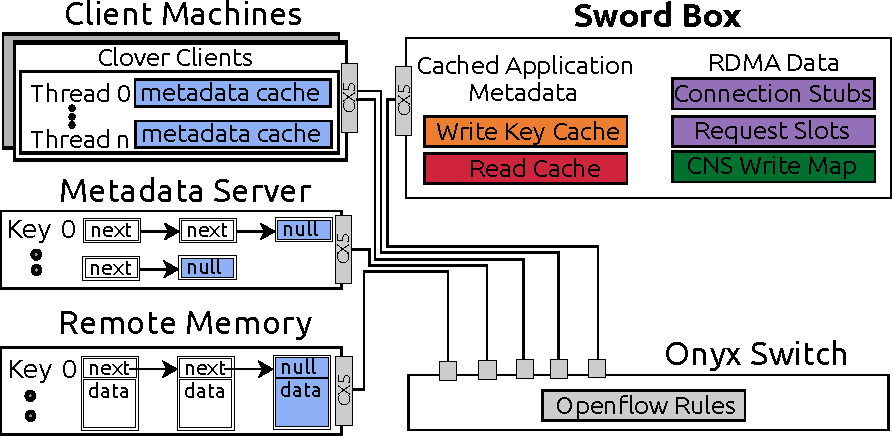
\includegraphics[width=0.45\textwidth]{fig/overview_2.pdf}
%%   %%
%%  \vskip 0.5em
%% \caption{Clients, Metadata and Remote Memory servers are
%% Clover components. {\sword} is run on a separate server connected to the same ToR.
%% Routing to {\sword} is effected by adding OpenFlow rules to redirect Clover traffic to \sword.
%% \todo{redo diagram}}
%% %%
%% \label{fig:overview} \end{figure}

% \sg{This might be where we should state that we did not build this part on the
% programmable switch.}

\subsection{Conflict avoidance}
\label{ca}

While atomic replacement can alleviate the NIC hardware bottleneck
that limits systems like Sherman, it does not address the underlying
contention for shared data structures.  Systems like Clover that
eschew locks in favor of optimistic concurrency therefore see little
benefit.  In these cases, however, \sword\ can have an even greater
impact by adjusting doomed-to-fail optimistic requests in flight, a process we term \emph{steering}.
%
%like Clover he single biggest impact
%an on-path serializer like {\sword} can have is to dramatically decrease the
%likelihood of a failed RDMA request due to a stale hint.  Specifically, because
%{\sword} can observe and modify operations as they go by, it can ``correct'' any
%requests it knows to be likely to fail.
Note that steering is strictly a performance
enhancement---because the requests continue to be (guarded by atomics
when necessary and) processed by the server as usual, any unexpected
reordering will cause the request to fail (and be retried by Clover),
just as it would have without rewriting.

%% Figure~\ref{fig:overview} shows how {\sword} interacts with systems
%% using cover as an example. Clover is implemented as a data path program written
%% in P4 and loaded onto a P4 TOR switch.  Client machines need not be directly
%% attached to the ToR, although they likely would be in most rack-scale
%% deployments.  Similarly, the topological location of Clover's metadata server is
%% irrelevant, but we expect it is also likely connected to the same switch.  For
%% the purposes of our discussion, we presume that {\sword} first places all
%% received RDMA requests into a total order before processing them; likewise
%% responses from a given server are totally ordered before processing.

\subsubsection{Write steering}

Recall that writes in Clover are destined to the presumed tail of a
key's linked list, but the target of any individual RDMA request may
be out of date due to races with concurrent updates.  Clover detects
concurrent updates by breaking writes (i.e., list appends) into two
RDMA operations: one write to create a new node, and a CAS operation
to update the next pointer of the node at the tail of the list---the
latter fails when another node was added concurrently.  To prevent
such stale CAS requests from failing, {\sword} maintains a cache of
the location of the (next pointer of the) node at the tail of each
key's linked list. If a CAS request arrives at {\sword} destined for a
stale virtual address (i.e., an address other than the one currently
cached for that key), {\sword} redirects the corresponding Clover
write request by replacing its target with the cached address.

%While conceptually simple, the actual implementation is somewhat
%involved due to the design of both Clover and the RDMA protocol and
%our desire to remain transparent to both.  Specifically,
Unfortunately, Clover RDMA CAS requests do not explicitly specify the
write operation of which they are a part.  {\sword} infers the
operation by checking the size of the RDMA request and then extracts
the key from the appropriate the location in the packet.  The key is
used as an index into a lookup table to find the virtual address of
the latest write for that key.  Our strategy requires 64 bytes of
data per key---the size of the RDMA virtual address.
%% Because it
%% modifies the content of the RDMA request, {\sword} also needs to
%% recompute the RDMA ICRC checksum to prevent the server from rejecting
%% the request as malformed.

%By
%performing this lookup in the data path all writes succeed regardless
%of how contested the memory address is. \todo{ref fig from words}.

\subsubsection{Read steering}

While Clover 
writes contain the key
to which they pertain---which allows for a table lookup---Clover's
RDMA read requests only contain the target virtual address and a size.
%When a
%read fails it must be retried, as mentioned earlier reads are
%performed iteratively until the tail of the list is reached, which in
%the case of highly contested keys could be arbitrarily long. Repeating
%reads does not destroy system performance as they are lockless,
%however in terms of client latency each retry adds serious
%latency. What makes handling reads hard is identifying the clover key
%for which the read is for, without additional data in the packet the
%value must be determined another way.
As reads can be for arbitrarily old virtual addresses a naive solution
that stored the lineage of each key would effectively require caching
the entire contents of Clover's metadata server.  Instead,
\sword\ hashes the address of each write into an array somewhat larger
than the size of the key space and stores the key along with the
address.  Collisions are resolved by replacing the old
%address
%and key with the new values
entry, allowing keys with higher update rates to
maintain longer histories in the table.

When reads arrive {\sword} looks up their destination address in the table; if
the address has a hit the associated key is used to look up the current tail in
the write cache and the RDMA read is steered to the cached location.  Should a
miss occur---either because the hash bucket was overwritten by another key, or
because the tail address is not cached---the read is left unmodified.  If it
fails to arrive at the current tail, Clover's recovery mechanism kicks in looks
up the last known address at the metadata server, then repeats the processes.


\subsection{Failure handling}

\sword\ collocates functionality---and therefore shares fate---with the
top-of-rack switch: if \sword\ fails, connectivity was already
disrupted (i.e., the ToR is down).  Hence, the fact that a
\sword\ failure will reset all remapped RDMA queue pairs to the
attached servers seems of little additional consequence.  In the case
of steering, however, we note that \sword\ does not maintain any hard
state: failure simply results in a performance hiccup if packet-level
connectivity can be maintained.  The upshot is that a complete
\sword\ failure does not introduce safety concerns in any event.

However, there are other failure scenarios to consider.  In
particular, we presume that the ToR sees the exact stream of packets
that will be received---and processed---by attached servers.
Unfortunately, this may not be true due to packet loss (e.g., due to
CRC failures or queue overflow) or even bugs on the server.  Of
course, these failure cases exist even without \sword, and Sherman and
Clover both provide their own error handling.  The key distinction,
however, is that \sword\ maintains a cache that may become
inconsistent with an attached server, which was previously the single
authority of both application and RDMA connection state.


At an application level, Clover never acquires any locks so failures
do not result in resource stranding, and Sherman periodically detects
if locks were kept by a dead client.  At the connection level they
both rely upon RDMA to provide reliable, in-order delivery of their
messages on a per-client basis and react to failed CAS operations by
retrying their operations.  {\sword} must therefore be able to detect
and properly handle packet retransmissions; in particular \sword\ must
not treat a retransmitted packet as a new operation.  Hence,
\sword\ tracks the most recent sequence number on each QP, the
transformation it applied (remapping or steering), and whether the
operation was ACK'd by the server.  Upon retransmission
\sword\ re-applies the previous transformation.

%QP ordering ensures retransmissions are , and RDMA
%go-back-$n$ is triggered if any message is lost.

\textbf{Enforcing ordering.}
Managing responses when mapping queue pairs is somewhat more complex.  If a
packet is dropped between \sword\ and a server and \sword\ maps a subsequent
request from a different client onto the same QP, the server will generate a
go-back-$n$ response and any other in-flight requests on that QP will become
invalidated.  Hence, when {\sword} sees a go-back-$n$ ACK, it triggers the same
mechanism used for ACK coalescing but in reverse: it broadcasts a go-back-$n$
ACK to all clients with outstanding messages.  While this approach amplifies the
performance impact of a lost packet, we expect such scenarios to be unlikely in
practice.  Indeed, no packet drops ever occurred between {\sword} and a server
during our experiments because our clients issue only closed-loop operations.

\textbf{Conflict avoidance.} Without queue-pair mapping, there are
fewer concerns at the connection level, but \sword\ must now be aware
of potential inconsistency between its cache and server state.
Concretely, in the case of Clover, it is possible for a linked list to
become ``broken''.  If \sword\ sees a client issue a \texttt{CAS(A,B)}
request (attempting to append node $B$ to the list at $A$) before
another issues \texttt{CAS(A,C)} (appending node $C$ to the
same---stale---tail), \sword\ will steer \texttt{CAS(A,C)} to
\texttt{CAS(B,C)}. If the \texttt{CAS(A,B)} operation is lost between
\sword\ and the server, \texttt{CAS(B,C)} will still succeed, causing
a broken chain: the pointer $A\rightarrow B$ does not exist but
$B\rightarrow C$ does, and {\sword} believes $C$ to be the tail.

In the normal case, the client will timeout and retransmit
\texttt{CAS(A,B)}, which \sword\ will identify as a retransmission and
\emph{not} steer to the ``new'' tail, thereby repairing the list.  (In
the mean time, the missing link is immaterial because
subsequent requests are being steered by \sword.)  If, however, the client
were to fail prior to retransmitting the CAS the chain will remain broken.
Here we use an out-of-band mechanism to repair the chain: on occasion
our control plane queries the switch to check for outstanding CAS
requests and simply retransmits them (spurious retransmissions are
handled gracefully by the server).  The trickiest case is if
\sword\ itself also fails in the mean time: we defer protecting
against this double-failure scenario to future work.

%\textbf{Connection Remapped Failures:} Unlike in the prior scenario, when
%connections are mapped no data corruption can occur.


%Note that because none of those operations were committed the order and
%completion of any client operations does not matter. Clients can fail
%independently without any concern for data structure safety.  

% Retransmission in this
% case is more complex. A single failed packet will require that all in-flight
% requests from all clients on that QP be retransmitted. If a single message is
% dropped, a following message will trigger a go-back-n response from the memory
% side NIC. We propagate the go-back-n message to all clients with outstanding
% requests using the same mechanism we use to repair coalesced acks, but in
% reverse.  Retransmit requests can be serviced in any order, as none had yet been
% delivered to memory, and if any clients die before retransmitting the structure
% remains safe in spite of their failure.

% One aspect which requires care is maintaining {\sword} state when dealing with
% go-back-n. In the case of Sherman, the value of the lock when a CAS is issued is
% stored in the request mapping stub. If go-back-n is invoked the state of the
% lock is reverted to the value it had just prior to issuing the failed request.
 

% Our goal is ensure that under failure \sword does not introduce any correctness
% issues. Clover ensures end-to-end correctness for packet failures and client
% failures. A key difference between default clover, and \sword enhanced Clover is
% a change in atomic domain. In clover atomic operations are executed by a memory
% side RDMA NIC, in \sword atomic decision are made at the switch. This
% introduces a potential for correctness issues if packets are lost between the
% switch, and memory server, and if clients fail during such events.

% The primary saftey issue introduced by \sword is a broken list. For example if a
% list A->B exists and there are outstanding writes C and D. If concurrent
% requests connect B->C and C->D but the CAS for B->C fails and C->D succeeds this
% creates a broken chain. Subsequent requests will be steered to the disconnected
% chain. One option would be to detect chain breakages and ask clients to reset by
% traversing the chain from root to tail. While tempting this approach could cause
% inconsistancies as clients might read and write data only to be notified of the
% link breakage further down the line. As such we task \sword with enforcing
% atomicity on lost CAS operations between itself and downstream memory servers.

% First we note that RDMA congestion control makes this problem an unlikely
% occurrence on a single hop. During testing we never witnessed packet drop
% between the switch egress port, and RDMA NIC, however corrupted packets, and
% drops could occur.

% If a packet is dropped between \sword and a memory servers NIC, the client will
% time out eventually and retry the operation. We track the last sequence number
% of each client CAS operation, and the virtual address it was steered to. As
% clients are closed loop this is limited to 88 bits per client connection. If we
% see that a client retries a CAS we steer that CAS to the same location it was
% steered to rather than the end of the list.

% In the less likely case that during a dropped packet a client dies, and fails to
% retry the chain could potentially remain disconnected indefinitely. To remedy
% this final case we keep an additional bit set on each client connection marked
% to 1 if a CAS has not been ACKd, and 0 otherwise. Periodically, or upon being
% notified of a client failure, our P4 control plane checks the state of client
% connections and sees if any outstanding CAS operations were never ACKed. If so
% \sword generates the dropped CAS from it's connection table information to
% reconnect the list.

% Note, it is only when CAS packets are dropped from \sword to memory that these
% precautions must be taken. Packets dropped prior to reaching \sword, and on the
% reverse path after operations are committed, and handled by RDMA's go-back-n and
% Clovers recovery mechanisms.



% Steering requests prior to the completion of CAS is safe in most cases while the
% switch is operating correctly and no client failures exist. However in subtle
% cases saftey violations can be introduced if proper measures are not taken. We
% take advantage of the fact that Clover has built in recovery mechanisms. When a
% failure is detected we rely on clover to recover by triggering it's default
% mechanism. By default when clover detects a failure, it traverses the list of
% keys recursively by issuing reads until it finds the new tail.


% \textbf{Cas fails due to not being the tail}
% In the common case B->C will never fail as the switch will steer requests to
% known successful locations. If a successful client request was not routed
% through {\sword} a CAS can return with a failed operation because it was not
% issued to the tail of the list. In this case {\sword} will see the failed
% response and begin by marking the key as invalid. All responses on that key will
% then be changed to failed CAS which will trigger Clovers recovery mechanism.
% \sg{On swordbox we have two options one of which is to examine the failed CAS,
% assuming that it was a correct write that CAS should point to the next valid
% location. Here the switch can simply update its value for the tail of the list
% to the next pointer of the failed CAS}. The second option is to clear the cache
% and then proactively wait for a successful CAS before steering again.

% \textbf{Packet is dropped after Swordbox, and before NIC processing}
% A trickier case in when the CAS operation for B->C is dropped prior to being
% processed by the NIC i.e the packet is dropped due to congestion. Typically this
% will not happen because the NIC generates pause frames before it becomes too
% congested, in our single TOR setup pause frames prevented packet drops due to
% the close loop design of clover. If the drop does occur however it is difficult
% to detect that the chain has been broken. In the common case the client which
% issued the CAS initially will retry. \sg{I did this on the dpdk box} If the same
% request is issued twice {\sword} could attempt to allow the packet to repair the
% broken chain by issuing it again, however this would incur significant buffering
% on the switch to track potentially lost packets. In the case of a retried CAS we
% mark the key a broken and force all clients to retry by marking their next CAS
% as failed.

% \textbf{Packet dropped, client failure}

% If a client's packet is dropped after \sword commits the CAS and the client
% fails before issuing another request, there is no retry to mark the key as
% invalid. In this case we need to refer to a timeout. On each key we keep a 32
% bit register used to mark outstanding requets. Each key also has a counter which
% counts the total number of CAS issued on the key. When a CAS is processed by
% \sword it increments the counter, and then marks a bit in the 32 bit counter
% modulo the packet counter. The number of the request is stored in the connection
% state of the client. When a response comes back on the client connection it the
% bit in the connection counter is set back to 0. When a CAS is issued, if the bit
% in our CAS tracker is set to 1, then a dropped CAS has been identified. In this
% case the key is marked as invalid and clients must attempt to retry the request.
% Out of band the client connections are checked by our control plane, if a rarely
% written key is unacked for a long period of time the key is marked as invalid
% Out of band the client connections are checked by our control plane, if a rarely
% written key is unacked for a long period of time the key is marked as invalid.

% \textbf{Client sends CAS, packet dropped before hitting the nic, and client
% dies/disconnects before retry}

% If a client cas fails, while another succeeds, and {\sword} also fails before
% being able to correct the fault clients the clients could be left in a state
% where some data is detached, and no mechanism which currently exists would
% detect the detachment. Here we suggest that if {\sword} fails clients trigger a
% \textit{read from the start} recovery to ensure that data remains consistent.


% \textbf{Read Steering}

% Reads also represent a tricky case upon write failure. If we use the same write
% tail to steer reads we can end up with inconsistent reads as they may be on a
% detached tail. Assuming that we will not attempt to repair the broken chain by
% inserting a write, the read is invalid.

% We can remedy this by only steering reads to locations that have had their CAS
% acked. This requires maintaining the write ack tail. And will come at the cost
% of performance. under contention.


% \subsubsection{Thoughts}

% \sg{A naive option would be to keep track of uncommited CAS, and then reissue
% them from the switch. This would defer the atomicity to the switch after it was
% effectivly atomicized by the switch. This is the definition of non-soft state
% though.}

% \sg{The key bit is that we can trigger a fault on all future calls to a broken key.}







